\hypertarget{TestStatistic_8c}{
\section{Test\-Statistic.c File Reference}
\label{TestStatistic_8c}\index{TestStatistic.c@{TestStatistic.c}}
}
{\tt \#include \char`\"{}party.h\char`\"{}}\par


Include dependency graph for Test\-Statistic.c:\begin{figure}[H]
\begin{center}
\leavevmode
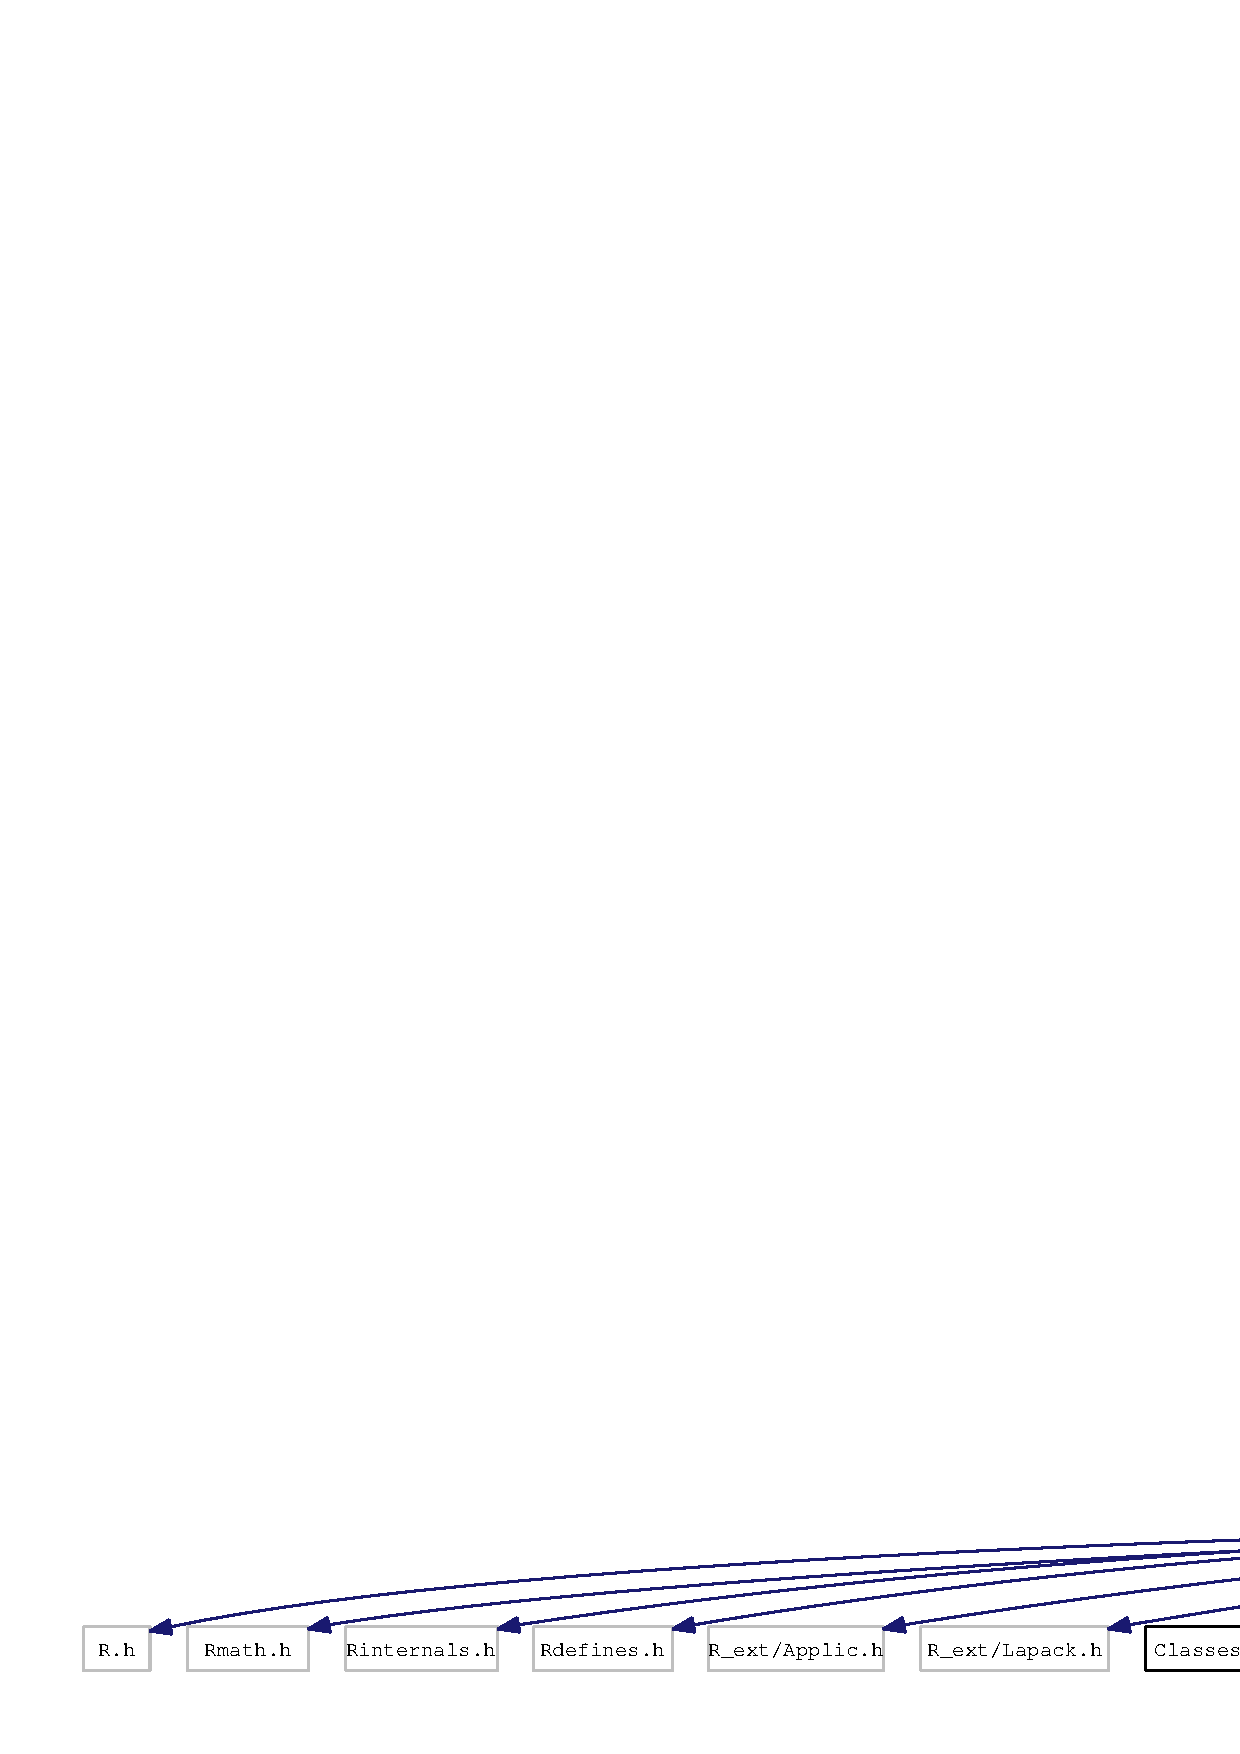
\includegraphics[width=172pt]{TestStatistic_8c__incl}
\end{center}
\end{figure}
\subsection*{Functions}
\begin{CompactItemize}
\item 
void \hyperlink{TestStatistic_8c_9ecf0700a00ad5fd64601bf718f20439}{C\_\-standardize} (const double $\ast$t, const double $\ast$mu, const double $\ast$Sigma, int pq, double tol, double $\ast$ans)
\item 
void \hyperlink{TestStatistic_8c_6939f019d2c7f42ae824776043a8c704}{C\_\-absstandardize} (const double $\ast$t, const double $\ast$mu, const double $\ast$Sigma, int pq, double tol, double $\ast$ans)
\item 
double \hyperlink{TestStatistic_8c_a3a1f48e4bb3aa19d1bac85a53358638}{C\_\-maxabs\-Test\-Statistic} (const double $\ast$t, const double $\ast$mu, const double $\ast$Sigma, int pq, double tol)
\item 
SEXP \hyperlink{TestStatistic_8c_499b26b98aaf073dc66135ecde8ad851}{R\_\-maxabs\-Test\-Statistic} (SEXP t, SEXP mu, SEXP Sigma, SEXP tol)
\item 
double \hyperlink{TestStatistic_8c_b45eb88ec3b2cc87e8610771cdcf53c4}{C\_\-quadform\-Test\-Statistic} (const double $\ast$t, const double $\ast$mu, const double $\ast$Sigma\-Plus, int pq)
\item 
SEXP \hyperlink{TestStatistic_8c_825d2b1db2c719f8d1c2e2ec3f79e1a4}{R\_\-quadform\-Test\-Statistic} (SEXP t, SEXP mu, SEXP Sigma\-Plus)
\end{CompactItemize}


\subsection{Detailed Description}
Test statistics for conditional inference

\begin{Desc}
\item[Author:]\begin{Desc}
\item[Author]hothorn \end{Desc}
\end{Desc}
\begin{Desc}
\item[Date:]\begin{Desc}
\item[Date]2005-06-14 11:21:32 +0200 (Tue, 14 Jun 2005) \end{Desc}
\end{Desc}


Definition in file \hyperlink{TestStatistic_8c-source}{Test\-Statistic.c}.

\subsection{Function Documentation}
\hypertarget{TestStatistic_8c_6939f019d2c7f42ae824776043a8c704}{
\index{TestStatistic.c@{Test\-Statistic.c}!C_absstandardize@{C\_\-absstandardize}}
\index{C_absstandardize@{C\_\-absstandardize}!TestStatistic.c@{Test\-Statistic.c}}
\subsubsection[C\_\-absstandardize]{\setlength{\rightskip}{0pt plus 5cm}void C\_\-absstandardize (const double $\ast$ {\em t}, const double $\ast$ {\em mu}, const double $\ast$ {\em Sigma}, int {\em pq}, double {\em tol}, double $\ast$ {\em ans})}}
\label{TestStatistic_8c_6939f019d2c7f42ae824776043a8c704}


Absolute values of standardized statistics \begin{Desc}
\item[Parameters:]
\begin{description}
\item[{\em t}]the vector of statistics \item[{\em mu}]expectations \item[{\em Sigma}]covariance matrix \item[{\em pq}]dimension of t \item[{\em tol}]tolerance for variances \item[{\em ans}]return value; a pointer to a REALSXP-vector of length pq \end{description}
\end{Desc}


Definition at line 49 of file Test\-Statistic.c.

References C\_\-abs(), and C\_\-standardize().

Referenced by C\_\-maxabs\-Test\-Statistic().

Here is the call graph for this function:\begin{figure}[H]
\begin{center}
\leavevmode
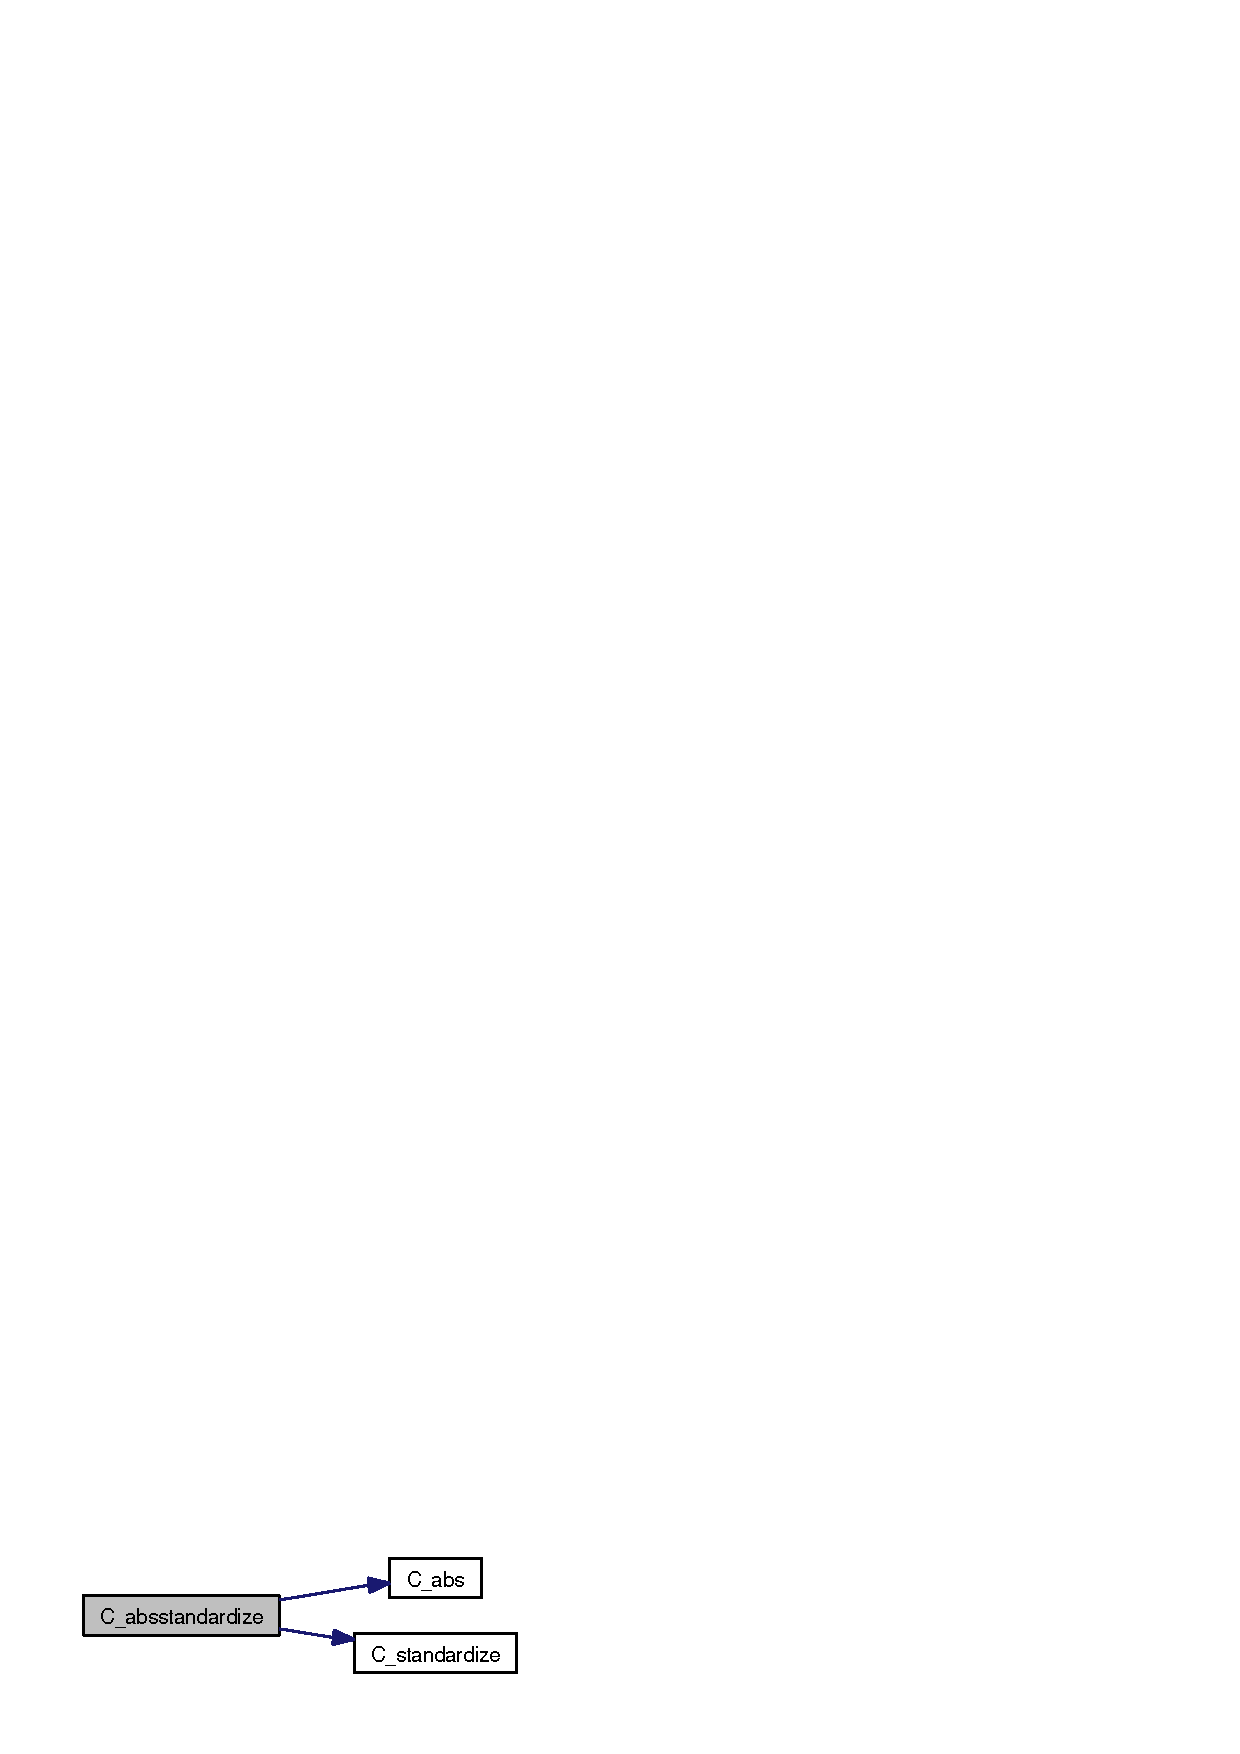
\includegraphics[width=126pt]{TestStatistic_8c_6939f019d2c7f42ae824776043a8c704_cgraph}
\end{center}
\end{figure}
\hypertarget{TestStatistic_8c_a3a1f48e4bb3aa19d1bac85a53358638}{
\index{TestStatistic.c@{Test\-Statistic.c}!C_maxabsTestStatistic@{C\_\-maxabsTestStatistic}}
\index{C_maxabsTestStatistic@{C\_\-maxabsTestStatistic}!TestStatistic.c@{Test\-Statistic.c}}
\subsubsection[C\_\-maxabsTestStatistic]{\setlength{\rightskip}{0pt plus 5cm}double C\_\-maxabs\-Test\-Statistic (const double $\ast$ {\em t}, const double $\ast$ {\em mu}, const double $\ast$ {\em Sigma}, int {\em pq}, double {\em tol})}}
\label{TestStatistic_8c_a3a1f48e4bb3aa19d1bac85a53358638}


Maximum absolute values of standardized statistics \begin{Desc}
\item[Parameters:]
\begin{description}
\item[{\em t}]the vector of statistics \item[{\em mu}]expectations \item[{\em Sigma}]covariance matrix \item[{\em pq}]dimension of t \item[{\em tol}]tolerance for variances \end{description}
\end{Desc}


Definition at line 66 of file Test\-Statistic.c.

References C\_\-absstandardize(), and C\_\-max().

Referenced by C\_\-Test\-Statistic(), and R\_\-maxabs\-Test\-Statistic().

Here is the call graph for this function:\begin{figure}[H]
\begin{center}
\leavevmode
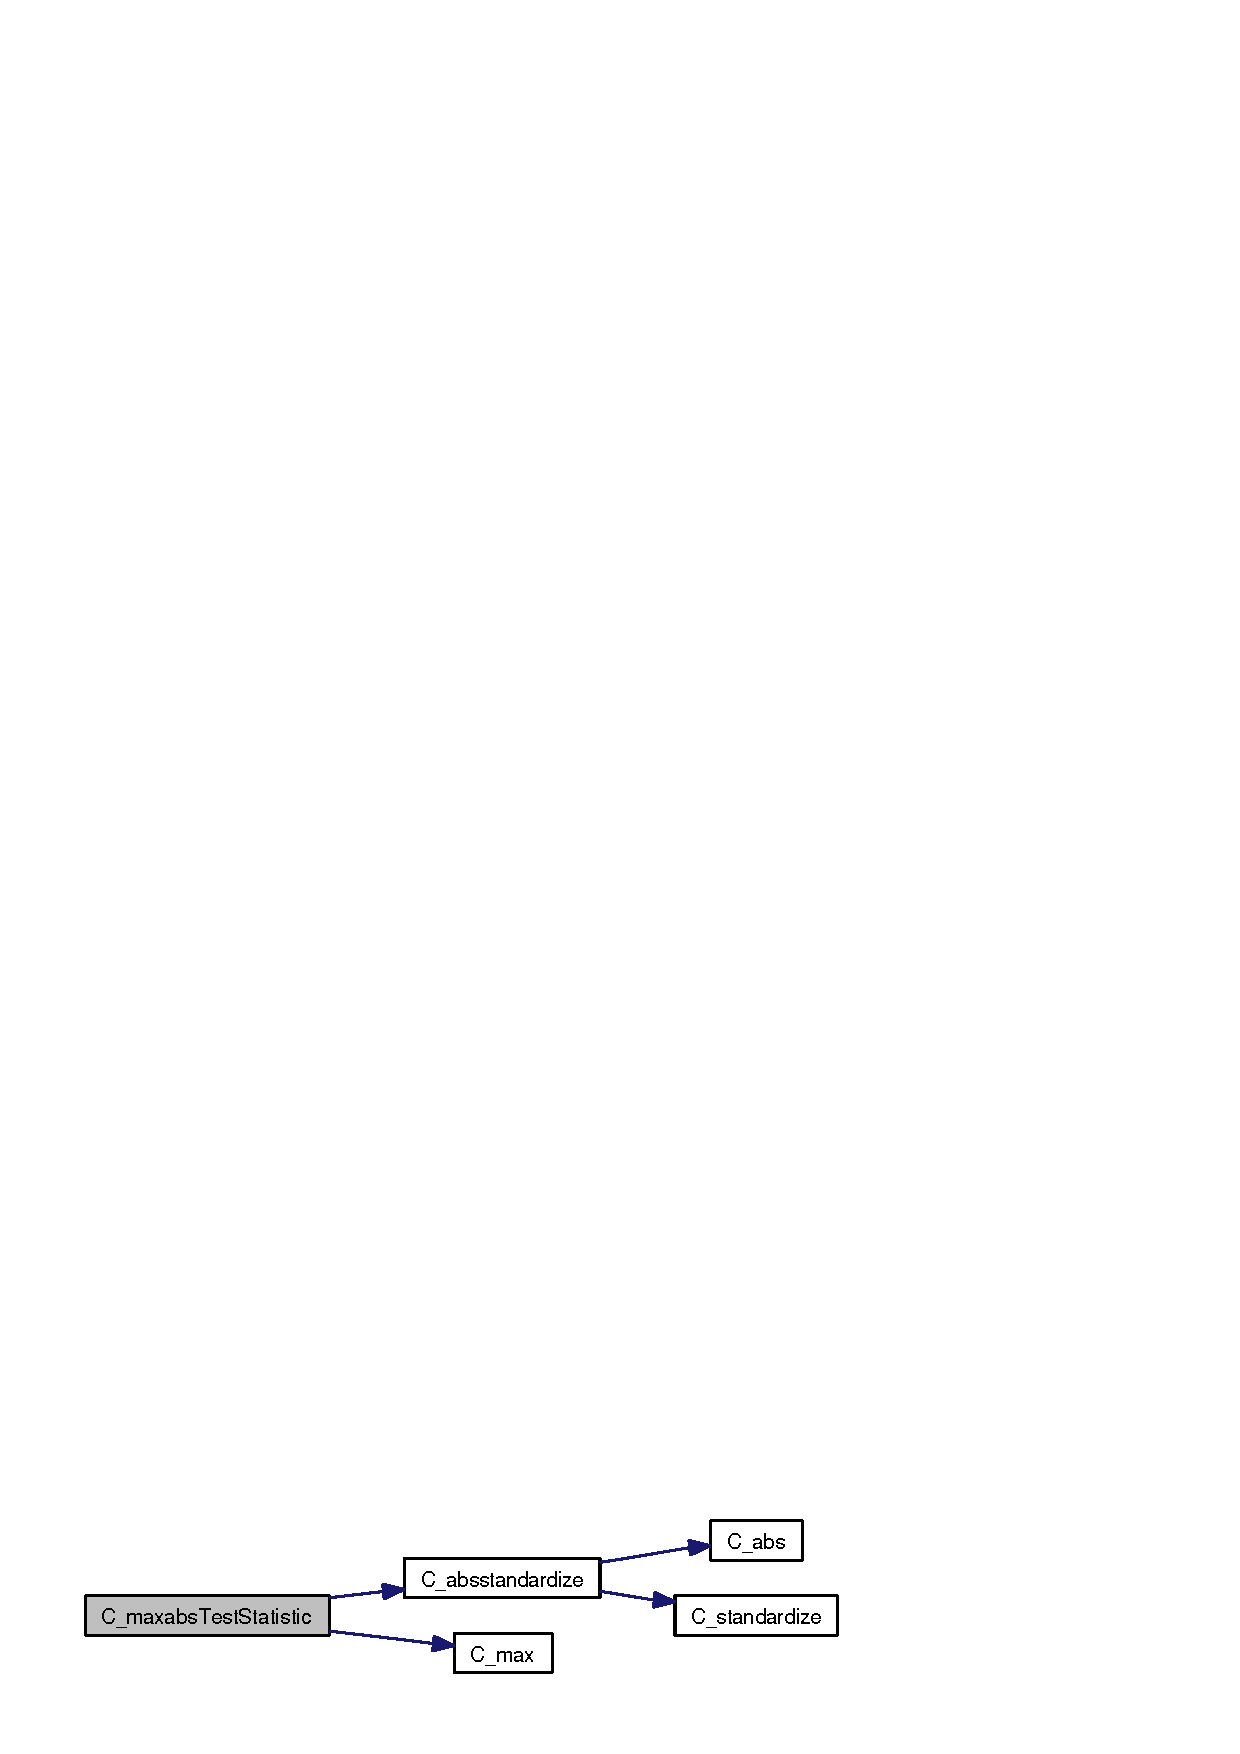
\includegraphics[width=204pt]{TestStatistic_8c_a3a1f48e4bb3aa19d1bac85a53358638_cgraph}
\end{center}
\end{figure}
\hypertarget{TestStatistic_8c_b45eb88ec3b2cc87e8610771cdcf53c4}{
\index{TestStatistic.c@{Test\-Statistic.c}!C_quadformTestStatistic@{C\_\-quadformTestStatistic}}
\index{C_quadformTestStatistic@{C\_\-quadformTestStatistic}!TestStatistic.c@{Test\-Statistic.c}}
\subsubsection[C\_\-quadformTestStatistic]{\setlength{\rightskip}{0pt plus 5cm}double C\_\-quadform\-Test\-Statistic (const double $\ast$ {\em t}, const double $\ast$ {\em mu}, const double $\ast$ {\em Sigma\-Plus}, int {\em pq})}}
\label{TestStatistic_8c_b45eb88ec3b2cc87e8610771cdcf53c4}


Quadratic form t(t - mu) Sigma\-Plus (t - mu) \par
 \begin{Desc}
\item[Parameters:]
\begin{description}
\item[{\em t}]the vector of statistics \item[{\em mu}]expectations \item[{\em Sigma\-Plus}]Moore-Penrose inverse \item[{\em pq}]dimension of t \end{description}
\end{Desc}


Definition at line 110 of file Test\-Statistic.c.

Referenced by C\_\-Test\-Statistic(), and R\_\-quadform\-Test\-Statistic().\hypertarget{TestStatistic_8c_9ecf0700a00ad5fd64601bf718f20439}{
\index{TestStatistic.c@{Test\-Statistic.c}!C_standardize@{C\_\-standardize}}
\index{C_standardize@{C\_\-standardize}!TestStatistic.c@{Test\-Statistic.c}}
\subsubsection[C\_\-standardize]{\setlength{\rightskip}{0pt plus 5cm}void C\_\-standardize (const double $\ast$ {\em t}, const double $\ast$ {\em mu}, const double $\ast$ {\em Sigma}, int {\em pq}, double {\em tol}, double $\ast$ {\em ans})}}
\label{TestStatistic_8c_9ecf0700a00ad5fd64601bf718f20439}


Standardizes a statistic t of length pq with mean mu and covariance Sigma for variances $>$ tol \par
 \begin{Desc}
\item[Parameters:]
\begin{description}
\item[{\em t}]the vector of statistics \item[{\em mu}]expectations \item[{\em Sigma}]covariance matrix \item[{\em pq}]dimension of t \item[{\em tol}]tolerance for variances \item[{\em ans}]return value; a pointer to a REALSXP-vector of length pq \end{description}
\end{Desc}


Definition at line 23 of file Test\-Statistic.c.

Referenced by C\_\-absstandardize(), C\_\-Node(), and R\_\-splitcategorical().\hypertarget{TestStatistic_8c_499b26b98aaf073dc66135ecde8ad851}{
\index{TestStatistic.c@{Test\-Statistic.c}!R_maxabsTestStatistic@{R\_\-maxabsTestStatistic}}
\index{R_maxabsTestStatistic@{R\_\-maxabsTestStatistic}!TestStatistic.c@{Test\-Statistic.c}}
\subsubsection[R\_\-maxabsTestStatistic]{\setlength{\rightskip}{0pt plus 5cm}SEXP R\_\-maxabs\-Test\-Statistic (SEXP {\em t}, SEXP {\em mu}, SEXP {\em Sigma}, SEXP {\em tol})}}
\label{TestStatistic_8c_499b26b98aaf073dc66135ecde8ad851}


R-interface to C\_\-maxabs\-Test\-Statistic \begin{Desc}
\item[Parameters:]
\begin{description}
\item[{\em t}]the vector of statistics \item[{\em mu}]expectations \item[{\em Sigma}]covariance matrix \item[{\em tol}]tolerance for variances \end{description}
\end{Desc}


Definition at line 87 of file Test\-Statistic.c.

References C\_\-maxabs\-Test\-Statistic().

Here is the call graph for this function:\begin{figure}[H]
\begin{center}
\leavevmode
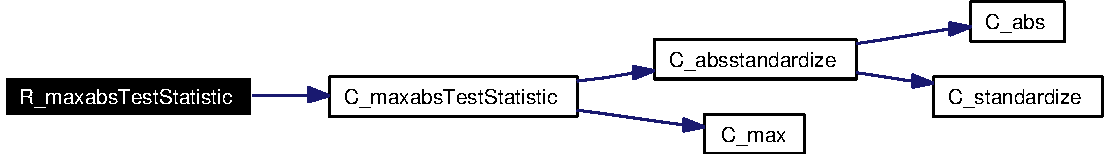
\includegraphics[width=282pt]{TestStatistic_8c_499b26b98aaf073dc66135ecde8ad851_cgraph}
\end{center}
\end{figure}
\hypertarget{TestStatistic_8c_825d2b1db2c719f8d1c2e2ec3f79e1a4}{
\index{TestStatistic.c@{Test\-Statistic.c}!R_quadformTestStatistic@{R\_\-quadformTestStatistic}}
\index{R_quadformTestStatistic@{R\_\-quadformTestStatistic}!TestStatistic.c@{Test\-Statistic.c}}
\subsubsection[R\_\-quadformTestStatistic]{\setlength{\rightskip}{0pt plus 5cm}SEXP R\_\-quadform\-Test\-Statistic (SEXP {\em t}, SEXP {\em mu}, SEXP {\em Sigma\-Plus})}}
\label{TestStatistic_8c_825d2b1db2c719f8d1c2e2ec3f79e1a4}


R-interface to C\_\-quadform\-Test\-Statistic \par
 \begin{Desc}
\item[Parameters:]
\begin{description}
\item[{\em t}]the vector of statistics \item[{\em mu}]expectations \item[{\em Sigma\-Plus}]Moore-Penrose inverse \end{description}
\end{Desc}


Definition at line 140 of file Test\-Statistic.c.

References C\_\-quadform\-Test\-Statistic().

Here is the call graph for this function:\begin{figure}[H]
\begin{center}
\leavevmode
\includegraphics[width=162pt]{TestStatistic_8c_825d2b1db2c719f8d1c2e2ec3f79e1a4_cgraph}
\end{center}
\end{figure}
